\documentclass{article}
\usepackage[utf8]{inputenc}
\usepackage{geometry}
\usepackage{fancyhdr}
\usepackage{titling}
\usepackage{datetime}
\usepackage{graphicx}
\usepackage{lipsum}
\usepackage{titlesec}
\usepackage{amsmath}
\usepackage{amssymb}
\usepackage{blkarray}

\usepackage{tikz}
\usetikzlibrary{automata, positioning}

% Set your name and assignment details here
\renewcommand{\author}{Taha Adeel Mohammed}
\newcommand{\rollnumber}{CS20BTECH11052}
\newcommand{\course}{AI3000/CS5500: Reinforcement Learning}
\newcommand{\assignment}{Assignment 1}

\renewcommand{\S}{\mathcal{S}}
\newcommand{\A}{\mathcal{A}}
\renewcommand{\P}{\mathcal{P}}
\newcommand{\R}{\mathcal{R}}
\newcommand{\Rhat}{\hat{\mathcal{R}}}

\renewcommand{\thesection}{Problem \arabic{section}:\!\!\!\!}
\renewcommand{\thesubsection}{(\alph{subsection})\!\!\!}
% \titleformat{\subsection}{\normalfont}{\thesubsection}{0.5em}{}

% Page setup
\geometry{a4paper, margin=1in}
\lfoot{\myname}
\rfoot{AI3000/CS5500}
\cfoot{\assignment}
\rfoot{\thepage}

% Title
\renewcommand{\maketitle}{
	\begin{center}
		\line(1,0){450} \\
		\vspace*{1ex}
        \Large{\textbf{\course}} \\
        \Large{\textbf{\assignment}} \\
    \end{center}
	\large{\author}
	\begin{flushright}
		\vspace*{-5ex}
		\rollnumber \\
	\end{flushright}
	\begin{center}
		\vspace*{-1ex}
		\line(1,0){450}
	\end{center}
}

\begin{document}

\maketitle

% Your content goes here

\section{Markov Reward process}
Consider a fair four sided dice with faces marked as {1, 2, 3, 4}. The dice is tossed repeatedly and independently. By formulating a suitable Markov reward process (MRP) and using Bellman equation for MRP, find the expected number of tosses required for the pattern '1234' to appear. Specifically, answer the following questions.

\subsection{Identify the states, transition probablities and terminal states (if any) of the MRP. (3 Points)}

We can formulate a Markov Process with the states $$\S = \{S_0, 1, 12, 123, 1234\},$$ where $S_0$ is the initial state and $1234$ is the terminal state. $1, 12, 123, 1234$ represent having gotten the sequence $1, 12, 123, 1234$ on consecutive die rolls respectively. The states with their transition probabilities are shown in the figure below.

\begin{figure}[h]
	\centering
	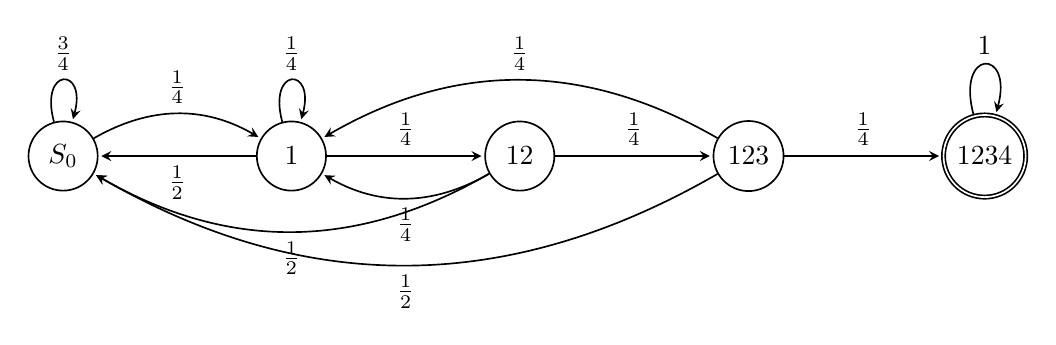
\begin{tikzpicture}[->,>=stealth,shorten >=1pt,auto,node distance=2cm,semithick]
		% Define the states
		\node[state] (S0) {$S_0$};
		\node[state, right=of S0] (1) {$1$};
		\node[state, right=of 1] (12) {$12$};
		\node[state, right=of 12] (123) {$123$};
		\node[state, right=of 123, accepting, double] (1234) {$1234$};
		
		% Define the transition probablities
		\path (S0) edge [loop above] node {$\frac{3}{4}$} (S0);
		\path (S0) edge [bend left] node {$\frac{1}{4}$} (1);
		\path (1) edge [loop above] node {$\frac{1}{4}$} (1);
		\path (1) edge node {$\frac{1}{2}$} (S0);
		\path (1) edge node {$\frac{1}{4}$} (12);
		\path (12) edge node {$\frac{1}{4}$} (123);
		\path (12) edge [bend left] node {$\frac{1}{4}$} (1);
		\path (12) edge [bend left] node {$\frac{1}{2}$} (S0);
		\path (123) edge node {$\frac{1}{4}$} (1234);
		\path (123) edge [bend right] node[above] {$\frac{1}{4}$} (1);
		\path (123) edge [bend left] node {$\frac{1}{2}$} (S0);
		\path (1234) edge [loop above] node {$1$} (1234);
	\end{tikzpicture}
	\caption{Markov Chain}
\end{figure}

\noindent
The transition probabilities are also shown in the matrix below: 
\vspace*{-1mm}
\begin{align}
	\P = \begin{blockarray}{cccccc}
	& \text{S0} & \text{1} & \text{12} & \text{123} & \text{1234} \\
	\begin{block}{c[ccccc]}
	\text{S0} & \frac{3}{4} & \frac{1}{4} & 0 & 0 & 0 \\
	\text{1} & \frac{1}{2} & \frac{1}{4} & \frac{1}{4} & 0 & 0 \\
	\text{12} & \frac{1}{2} & \frac{1}{4} & 0 & \frac{1}{4} & 0 \\
	\text{123} & \frac{1}{2} & \frac{1}{4} & 0 & 0 & \frac{1}{4} \\
	\text{1234} & 0 & 0 & 0 & 0 & 1 \\
	\end{block}
	\end{blockarray}
\end{align}
	
\subsection{Construct a suitable reward function, discount factor and use the Bellman equation for MRP to find the 'average' number of tosses required for the pattern '1234' to appear. (7 Points)}

We assign a reward of $-1$ to each of the states $S_0, 1, 12, 123$ and a reward of $0$ to the terminal state $1234$. i.e 
\begin{align}
	\R(s) = \begin{cases}
		-1 & \text{if } s \in \{S_0, 1, 12, 123\} \\
		0 & \text{if } s = 1234
	\end{cases}
\end{align}

We also set the discount factor $\gamma = 1$. This way, -$V(s)$ would represent the expected number of tosses required to reach the terminal state $1234$ from state $s$. Hence our required answer of average number of tosses required for the pattern $'1234'$ to appear is $-V(S_0)$.

\,\\
The Bellman equation for MRP is given by:
\begin{align}
	V(s) &= \R(s) + \gamma \sum_{s' \in \S} \P(s, s') V(s')
\end{align}

\noindent
Therefore, we have:
\begin{align}
	V(S_0) &= -1 + \frac{3}{4} V(S_0) + \frac{1}{4} V(1) \\
	V(1) &= -1 + \frac{1}{2} V(S_0) + \frac{1}{4} V(1) + \frac{1}{4} V(12) \\
	V(12) &= -1 + \frac{1}{2} V(S_0) + \frac{1}{4} V(1) + \frac{1}{4} V(123) \\
	V(123) &= -1 + \frac{1}{2} V(S_0) + \frac{1}{4} V(1) + \frac{1}{4} V(1234) \\
	V(1234) &= 0
\end{align}

\noindent
Solving the above equations, we get:
\begin{align*}
	V(S_0) &= -256, &
	V(1) &= -252, &
	V(12) &= -240, &
	V(123) &= -192, &
	V(1234) &= 0 &
\end{align*}

\noindent
Therefore, the average number of tosses required for the pattern $'1234'$ to appear is given by $-V(S_0) =\ \boxed{256 \text{ tosses.}}$

\,

\section{Markov Decision Process}
\subsection{Let M be an infinite horizon MDP given by $< \S, \A, \P, \R, \gamma >$ with $|\S| < \infty$ and $|\A| < \infty$ and $\gamma \in [0, 1)$. Suppose that the reward function $\R^a_{ss'}$ for any successor states $s, s' \in \S$ and action $a \in \A$ is non-negative and bounded, what is the lower and upper bound on the discounted sum of rewards? (3 Points)}


The discounted sum of rewards is given by:
\begin{align}
	G_t = \sum_{k=0}^\infty \gamma^k r_{t+k+1}
\end{align}

\noindent
Hence the least possible $G_t$ theoretically obtainable, i.e. a lower bound on $G_t$ is when for all $k \geq 0$, $r_{t+k+1} = r_{min} = min(\R^a_{ss'})\ \forall \ a \in \A$ and $s, s' \in \S$, which exists because the reward function is non-negative (and hence lower-bounded by 0). Therefore, we have:
\begin{align} 
	\boxed{G_t \geq \sum_{k=0}^\infty \gamma^k r_{min} = \frac{r_{min}}{1 - \gamma} }
\end{align}

\pagebreak
\noindent
Similarly, the upper bound on $G_t$ occurs when $\forall \ k \geq 0$, $r_{t+k+1} = r_{max} = max(\R^a_{ss'})$ $\forall \ a \in \A$ and $s, s' \in \S$, which exists because the reward function is bounded. Therefore, we have:
\begin{align}
	\boxed{G_t \leq \sum_{k=0}^\infty \gamma^k r_{max} = \frac{r_{max}}{1 - \gamma} }	
\end{align}
\,

\subsection{Let $\hat{M} = < \S, \A, \P, \Rhat, \gamma >$ be another infinite horizon MDP with a modified reward function $\Rhat$ such that $$\R^a_{ss'} - \Rhat^a_{ss'} = \epsilon,$$ where $\epsilon$ is a constant independent of $s \in \S$ or $a \in \A$. Given a policy $\pi$, let $V^\pi$ and $ \hat{V}^\pi$ be value functions of policy $\pi$ for MDPs $M$ and $\hat{M}$ respectively. Derive an expression that relates $V^\pi (s)$ to $\hat{V}^\pi (s)$ for any state $s \in \S$ of the MDP. (3 Points)}

We know that the value function $V^\pi(s)$ is given by:
\begin{align}
	V^\pi(s) &= E_\pi \left[ \sum_{k=0}^\infty \gamma^k r_{t+k+1} \bigg| s_t = s \right]
\end{align}
Since the reward function $\R^a_{ss'}$ is modified by a constant $\epsilon$ for all $s \in \S$ and $a \in \A$, using linearity of expectation, we have:
\begin{align}
	V^\pi(s) &= E_\pi \left[ \sum_{k=0}^\infty \gamma^k \left( \Rhat^a_{ss'} + \epsilon \right) \bigg| s_t = s \right] \\
	&= E_\pi \left[ \sum_{k=0}^\infty \gamma^k \Rhat^a_{ss'} \bigg| s_t = s \right] + E_\pi \left[ \sum_{k=0}^\infty \gamma^k \epsilon \bigg| s_t = s \right] \\
	&= E_\pi \left[ \sum_{k=0}^\infty \gamma^k \Rhat^a_{ss'} \bigg| s_t = s \right] + \epsilon \sum_{k=0}^\infty \gamma^k \\
	&= \hat{V}^\pi(s) + \frac{\epsilon}{1 - \gamma}
\end{align}

\noindent
Therefore we have:
\begin{align}
	\boxed{\implies V^\pi(s) - \hat{V}^\pi(s) = \frac{\epsilon}{1 - \gamma}}
\end{align}

\,

% We know that the value functions $V^\pi(s)$ and $\hat{V}^\pi(s)$ are given by:
% \begin{align}
% 	V^\pi(s) &= \sum_{a \in \A} \pi(a|s) \sum_{s' \in \S} \P(s, a, s') \left[ \R^a_{ss'} + \gamma V^\pi(s') \right] \\
% 	\hat{V}^\pi(s) &= \sum_{a \in \A} \pi(a|s) \sum_{s' \in \S} \P(s, a, s') \left[ \Rhat^a_{ss'} + \gamma \hat{V}^\pi(s') \right]
% \end{align}

% \pagebreak
% \noindent
% In above equations, the only difference is in the reward functions $\R^a_{ss'}$ and $\Rhat^a_{ss'}$. Therefore, subracting the two equations, we get:
% \begin{align}
% 	V^\pi(s) - \hat{V}^\pi(s) &= \sum_{a \in \A} \pi(a|s) \sum_{s' \in \S} \P(s, a, s') \left[ \R^a_{ss'}\! -\! \Rhat^a_{ss'} + \gamma \left( V^\pi(s') - \hat{V}^\pi(s') \right) \right] \\
% 	&= \sum_{a \in \A} \pi(a|s) \sum_{s' \in \S} \P(s, a, s') \left[ \epsilon + \gamma \left( V^\pi(s') - \hat{V}^\pi(s') \right) \right] \\
% 	&= \epsilon\!\sum_{a \in \A}\!\pi(a|s)\!\sum_{s' \in \S}\!\P(s,\!a,\!s')\!+\!\gamma\!\sum_{a \in \A}\!\pi(a|s)\!\sum_{s' \in \S}\!\P(s,\!a,\!s')\!\left(\!V^\pi(s')\!-\!\hat{V}^\pi(s')\!\right) \\
% 	&= \epsilon + \gamma \sum_{a \in \A} \pi(a|s) \sum_{s' \in \S} \P(s, a, s') \left( V^\pi(s') - \hat{V}^\pi(s') \right) \\
% 	&= \epsilon + \gamma \sum_{s' \in \S} \left( V^\pi(s') - \hat{V}^\pi(s') \right) \sum_{a \in \A} \pi(a|s) \P(s, a, s') \\
% 	&= \epsilon + \gamma \sum_{s' \in \S} \left( V^\pi(s') - \hat{V}^\pi(s') \right) \P^\pi(s, s') \\
% 	&= \epsilon + \gamma (V^\pi(s) - \hat{V}^\pi(s))
% \end{align}
% Therefore we have:
% \begin{align}
% 	\boxed{\implies V^\pi(s) - \hat{V}^\pi(s) = \frac{\epsilon}{1 - \gamma}}
% \end{align}
% \,

\subsection{Does $M$ and $\hat{M}$ have the same optimal policy ? Explain. (3 Points)}

Yes, $M$ and $\hat{M}$ have the same optimal policy. This is because the optimal policy $\pi^*$ is the one that maximizes the value function $V^{\pi^*}(s)$ for all $s \in \S$. Since we have shown in sub-question (b) that $V^{\pi^*}(s)$ and $\hat{V}^{\pi^*}(s)$ are related by a constant, therefore the optimal policy is the same, as the same action at each state would maximize both value functions $V^{\pi^*}(s)$ and $\hat{V}^{\pi^*}(s)$.

\, \\
\noindent
Mathematically, we can see this using the policy iteration method. We start with an initial policy $\pi_0$ and iteratively update it until we arrive at the optimal policy $\pi^*$. In each update for $M$, we have:
\begin{align}
	\pi_{k+1}(a|s) &= \begin{cases}
		1 & \text{if } a = \arg\max_{a \in \A} \sum_{s' \in \S} \P^a_{ss'} \left[ \R^a_{ss'} + \gamma V^{\pi_k}(s') \right] \\
		0 & \text{otherwise}
	\end{cases}
\end{align}

\noindent
Similarly, for $\hat{M}$, we have the update:
\begin{align}
	\hat{\pi}_{k+1}(a|s) &= \begin{cases}
		1 & \text{if } a = \arg\max_{a \in \A} \sum_{s' \in \S} \P^a_{ss'} \left[ \Rhat^a_{ss'} + \gamma \hat{V}^{\pi_k}(s') \right] \\
		0 & \text{otherwise}
	\end{cases} \\
	\implies \hat{\pi}_{k+1}(a|s) &= \begin{cases}
		1 & \text{if } a = \arg\max_{a \in \A} \sum_{s' \in \S} \P^a_{ss'} \left[ \R^a_{ss'} + \gamma (V^{\pi_k}(s') - \frac{\epsilon}{1-\gamma}) \right] \\
		0 & \text{otherwise}
	\end{cases} \\
	\implies \hat{\pi}_{k+1}(a|s) &= \begin{cases}
		1 & \text{if } a = \arg\max_{a \in \A} \sum_{s' \in \S} \P^a_{ss'} \left[ \R^a_{ss'} + \gamma V^{\pi_k}(s') \right] \\
		0 & \text{otherwise}
	\end{cases} \\
	\implies \hat{\pi}_{k+1}(a|s) &= \pi_{k+1}(a|s)
\end{align}

\, \\
Hence we can see that after each iteration of the policy iteration method, the policy $\pi_{k+1}$ for $M$ and $\hat{\pi}_{k+1}$ for $\hat{M}$ are the same. Therefore, the optimal policy $\pi^*$ for $M$ and $\hat{\pi}^*$ for $\hat{M}$ are also the same.

\,

\subsection{From sub-question (b) can one argue that the assumption that the MDP $M$ in sub-question (a) has non-negative and bounded reward is without loss in generality ? What if the MDP $M$ is allowed to have negative but bounded rewards ? (3 Points)}

Yes, the assumption that the MDP $M$ in sub-question (a) has non-negative and bounded reward is without loss in generality, as we have shown in sub-question (b) that the optimal policy is the same for both MDPs $M$ and $\hat{M}$, even if the reward function of $M$ is modified by a constant $\epsilon$. Hence for reward functions with negative but bounded rewards, we can simply add a constant $\epsilon$ to the reward function to make it non-negative and bounded, and the optimal policy would still be the same.

\,

\subsection{State and prove an analogous result for the sub-question (b) for the case when $M$ and $\hat{M}$ are finite horizon MDPs with horizon length $H < \infty$. (4 Points)}

The value function for a finite horizon MDP $M$ is given by:
\begin{align}
	V^\pi(s) &= E_\pi \left[ \sum_{k=0}^{H} \gamma^k r_{t+k+1} \bigg| s_t = s \right]
\end{align}

\noindent
Similarly to sub-question (b), since the reward function $\R^a_{ss'}$ is modified by a constant $\epsilon$ for all $s \in \S$ and $a \in \A$, we have:
\begin{align}
	V^\pi(s) &= E_\pi \left[ \sum_{k=0}^{H} \gamma^k \left( \Rhat^a_{ss'} + \epsilon \right) \bigg| s_t = s \right] \\
	&= E_\pi \left[ \sum_{k=0}^{H} \gamma^k \Rhat^a_{ss'} \bigg| s_t = s \right] + E_\pi \left[ \sum_{k=0}^{H} \gamma^k \epsilon \bigg| s_t = s \right] \\
	&= E_\pi \left[ \sum_{k=0}^{H} \gamma^k \, \Rhat^a_{ss'} \bigg| s_t = s \right] + \epsilon \sum_{k=0}^{H} \gamma^k \\
	&= \hat{V}^\pi(s) + \frac{\epsilon \, (1 - \gamma^{H+1})}{1 - \gamma}
\end{align}

\noindent
Therefore we have:
\begin{align}
	\boxed{\implies V^\pi(s) - \hat{V}^\pi(s) = \frac{\epsilon \, (1 - \gamma^{H+1})}{1 - \gamma}}
\end{align}

\,

\subsection{Now, consider an indefinite MDP or a stochastic shortest path MDP where the horizon length $H$ can vary. A subset of the state space $S_{term} \subset \S$ is considered terminal if a trajectory of the form $s_0, a_0, r_1, s_1, a_1, r_2, \cdots,$ keeps rolling out until a terminal state $S_H \in \S$ term is visited. In general, the length of the episode $H$ is a random variable. Does the analogous result of sub-question (b) hold when $M$ and $\hat{M}$ are indefinite MDPs ? Explain. (4 Points)}

For an indefinite MDP, with a varying horizon length $H$, the value function is given by:
\begin{align}
	V^\pi(s) &= E_\pi \left[ \sum_{k=0}^{H} \gamma^k r_{t+k+1} \bigg| s_t = s \right]
\end{align}

\noindent
Since the reward function $\R^a_{ss'}$ is modified by a constant $\epsilon$ for all $s \in \S$ and $a \in \A$, we have:
\begin{align}
	V^\pi(s) &= E_\pi \left[ \sum_{k=0}^{H} \gamma^k \left( \Rhat^a_{ss'} + \epsilon \right) \bigg| s_t = s \right] \\
	&= E_\pi \left[ \sum_{k=0}^{H} \gamma^k \Rhat^a_{ss'} \bigg| s_t = s \right] + E_\pi \left[ \sum_{k=0}^{H} \gamma^k \epsilon \bigg| s_t = s \right] \\
	&= E_\pi \left[ \sum_{k=0}^{H} \gamma^k \, \Rhat^a_{ss'} \bigg| s_t = s \right] + \epsilon \sum_{k=0}^{H} \gamma^k \\
	&= \hat{V}^\pi(s) + \frac{\epsilon \, (1 - \gamma^{H+1})}{1 - \gamma}
\end{align}

\noindent
Therefore we have:
\begin{align}
	\boxed{\implies V^\pi(s) - \hat{V}^\pi(s) = \frac{\epsilon \, (1 - \gamma^{H+1})}{1 - \gamma}}
\end{align}

\noindent
Therefore no, the analogous result of sub-question (b) does not hold when $M$ and $\hat{M}$ are indefinite MDPs, as the horizon length $H$ is not fixed, and hence the value functions $V^\pi(s)$ and $\hat{V}^\pi(s)$ are not related by a constant. 
\,

\subsection{For this sub-question, let $\hat{M} = < \S, \A, \P, \Rhat, \gamma >$ be a infinite horizon MDP with a modified reward function $\Rhat$ such that $$ \R^a_{ss'} - \Rhat^a_{ss'} \leq \epsilon $$ where $\epsilon$ is a constant independent of $s$ and $a$. Derive an expression that relates the optimal value functions $V_* (s)$ to $\hat{V}_* (s)$. Would $M$ and $\hat{M}$ have the same optimal policy ? Explain. (6 Points)}

Similar to sub-question (b), we claim that $V_*(s)$ and $\hat{V}_*(s)$ are related by:
\begin{align}
	V_*(s) - \hat{V}_*(s) \leq \frac{\epsilon}{1 - \gamma}
\end{align}

\noindent
\textbf{Proof by Induction: (Value Iteration Method)} \\
We start with an initial value function $V_0(s) = 0 \text{ and } \hat{V}_0(s) = 0 \ \forall \ s \in \S$. Then we iteratively update these value functions using the Value Iteration Method until we arrive at the optimal value functions $V_*(s)$ and $\hat{V}_*(s)$. \\

\noindent
\textbf{Base Case:} $V_0(s)- \hat{V}_0(s) = 0 \leq \frac{\epsilon}{1 - \gamma} \ \forall \ s \in \S$. \\

\noindent
\textbf{Induction Hypothesis:} $V_k(s) - \hat{V}_k(s) \leq \frac{\epsilon}{1 - \gamma} \ \forall \ s \in \S$, where $V_k$ and $\hat{V}_k$ are the value functions after $k$ iterations of the Value Iteration Method. \\

\noindent
\textbf{Induction Step:} We know that the value functions $V_{k+1}(s)$ and $\hat{V}_{k+1}(s)$ are given by:
\begin{align}
	V_{k+1}(s) &= \max_{a \in \A} \left[\sum_{s' \in \S} \P^a_{ss'}\left(\R^a_{ss'} + \gamma V_k(s')\right) \right] \\
	\hat{V}_{k+1}(s) &= \max_{a \in \A} \left[\sum_{s' \in \S} \P^a_{ss'}\left(\Rhat^a_{ss'} + \gamma \hat{V}_k(s')\right) \right]
\end{align}

\noindent
Note that these two equations might be maximized by different actions $a_1, a_2 \in \A$. However
\begin{align}
	\max_{a \in \A} f(a) - \max_{a \in \A} g(a) \leq \max_{a \in \A} \left[ f(a) - g(a) \right]
\end{align}

\noindent
Therefore by subracting the two equations, and utilising above inequality and our induction hypothesis, we get:
\begin{align*}
	V_{k+1}(s) - \hat{V}_{k+1}(s) &\leq \max_{a \in \A} \left[\sum_{s' \in \S} \P^a_{ss'}\left(\R^a_{ss'} + \gamma V_k(s')\right) \right] - \max_{a \in \A} \left[\sum_{s' \in \S} \P^a_{ss'}\left(\Rhat^a_{ss'} + \gamma \hat{V}_k(s')\right) \right] \\
	&\leq \max_{a \in \A} \left[\sum_{s' \in \S} \P^a_{ss'}\left(\R^a_{ss'} + \gamma V_k(s')\right) - \sum_{s' \in \S} \P^a_{ss'}\left(\Rhat^a_{ss'} + \gamma \hat{V}_k(s')\right) \right] \\
	&\leq \max_{a \in \A} \left[\sum_{s' \in \S} \P^a_{ss'}\left(\R^a_{ss'} - \Rhat^a_{ss'} + \gamma \left( V_k(s') - \hat{V}_k(s') \right) \right) \right] \\
	&\leq \max_{a \in \A} \left[\sum_{s' \in \S} \P^a_{ss'}\left(\epsilon + \gamma \left( V_k(s') - \hat{V}_k(s') \right) \right) \right] \\
	&\leq \max_{a \in \A} \left[\sum_{s' \in \S} \P^a_{ss'}\left(\epsilon + \gamma \frac{\epsilon}{1 - \gamma} \right) \right] \\
	&\leq \max_{a \in \A} \left[\sum_{s' \in \S} \P^a_{ss'}\left(\frac{\epsilon}{1 - \gamma} \right) \right] 
	= \frac{\epsilon}{1 - \gamma}
\end{align*}

\noindent
Therefore we have:
\begin{align}
	\boxed{\implies V_{k+1}(s) - \hat{V}_{k+1}(s) \leq \frac{\epsilon}{1 - \gamma}}
\end{align}

\noindent
Hence by by the principle of mathematical induction, we have:
\begin{align}
	\boxed{\implies V_*(s) - \hat{V}_*(s) \leq \frac{\epsilon}{1 - \gamma}}
\end{align}

\noindent
\textbf{Optimal Policy for $M$ and $\hat{M}$:} \\
$M$ and $\hat{M}$ need \textbf{not} have the same optimal policy. The modification in the reward function may affect the optimal policy, especially if the original optimal policy was sensitive to the exact reward values or the $\epsilon$ value is huge. Also in above calculations, we have seen that the optimal value functions can have different actions $a_1, a_2 \in \A$ that maximize them. Hence the optimal policy for $M$ and $\hat{M}$ may be different.

\,

\subsection{Now consider the MDP $M$ of sub-question (a). Does scaling the discount factor by a constant $\kappa \in (0, 1)$ alter the optimal policy ? Explain. (4 Points)}

\textbf{Yes,} scaling the discount factor by a constant $\kappa \in (0, 1)$ might alter the optimal policy. For example, it could convert an agent from a far-sighted agent to a myopic agent, or vice-versa. 

\, \\
For example, consider the below infinite horizon MDP $M$, with the original discount factor $\gamma = 0.5$. The image below shows the states of the MDP, with each arrow representing an action that will deterministically take them to the next state, and the reward $\R(s, a, s')$ associated with the transition shown on the arrow.

\begin{figure}[h]
	\centering
	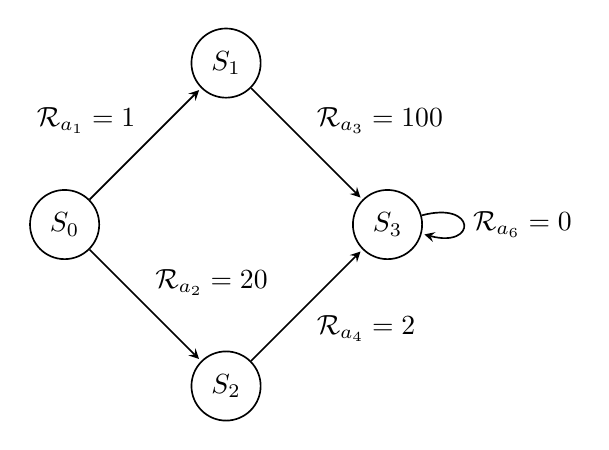
\begin{tikzpicture}[->,>=stealth,shorten >=1pt,auto,node distance=2cm,semithick]
		% Define the states
		\node[state] (S0) {$S_0$};
		\node[state, above right=of S0] (S1) {$S_1$};
		\node[state, below right=of S0] (S2) {$S_2$};
		\node[state, below right=of S1] (S3) {$S_3$};
		
		% Define the paths
		\path (S0) edge node {$\R_{a_1} = 1$} (S1);
		\path (S0) edge node {$\R_{a_2} = 20$} (S2);
		\path (S1) edge node {$\R_{a_3} = 100$} (S3);
		\path (S2) edge node[below right] {$\R_{a_4} = 2$} (S3);
		\path (S3) edge [loop right] node {$\R_{a_6} = 0$} (S3);
	\end{tikzpicture}
\end{figure}

\noindent
For $\gamma = 0.5$, for policy $\pi_1 = \{a_1, a_3, a_6, a_6, \cdots\}$ and $\pi_2 = \{a_2, a_4, a_6, a_6, \cdots\}$, we have:
\begin{align*}
	Q^{\pi_1}(S_0, a_1) &= 1 + 0.5 \times 100 + 0 + \ldots = 51 \\
	Q^{\pi_1}(S_0, a_2) &= 20 + 0.5 \times 2 + 0 + \ldots = 21  \\
	\therefore \pi^* = \pi_1 &= \underset{{a \in \A}}{\text{argmax}}\ Q^{\pi_1}(S_0, a) = a_1
\end{align*}

\noindent
However, if we scale gamma by $\kappa = 0^+$, i.e. $\gamma' \rightarrow 0$, then for policy $\pi_1 = \{a_1, a_3, a_6, a_6, \cdots\}$ and $\pi_2 = \{a_2, a_4, a_6, a_6, \cdots\}$, we have:
\begin{align*}
	Q^{\pi_1}(S_0, a_1) &= 1 + 0 \times 100 + 0 + \ldots = 1 \\
	Q^{\pi_1}(S_0, a_2) &= 20 + 0 \times 2 + 0 + \ldots = 20  \\
	\therefore \pi^* = \pi_2 &= \underset{{a \in \A}}{\text{argmax}}\ Q^{\pi_2}(S_0, a) = a_2
\end{align*}

\noindent
Therefore, scaling the discount factor by a constant $\kappa \in (0, 1)$ can alter the optimal policy.



\end{document}
